%!TEX encoding = UTF-8 Unicode
%
%  $Description: INESC ID
%
%  $Author:  
%  $Date: 
%  $Revision: 
%  
\documentclass{llncs}
%Numering
\pagestyle{plain} 
\RequirePackage[english]{babel} % Se fizerem o texto em ingles

\usepackage[utf8]{inputenc}
\usepackage{indentfirst}	%index allways the first paragraph
\usepackage{graphicx}  % allows for indexgeneration
\usepackage{subfig}  % allows for indexgeneration
\usepackage{amsmath} %math symbols
\usepackage{rotating} %rotate figure
\usepackage[nolist]{acronym} 	         % acronimos \usepackage
\usepackage{float}
\graphicspath{{eps/}{png/}}
\usepackage{color}
\usepackage{multirow}
%Marks on table
\usepackage{pifont}% http://ctan.org/pkg/pifont
\newcommand{\cmark}{\ding{51}}%
\newcommand{\xmark}{\ding{55}}%

%Section Reference: \cref{sec:foo}
\usepackage{cleveref}
\crefname{section}{§}{§§}

\usepackage{array}
\newcolumntype{C}[1]{>{\centering\arraybackslash}m{#1}}

\usepackage{rotating}
%Color on table
\usepackage[table]{xcolor}
\definecolor{lightgray}{gray}{0.9}
\usepackage{multirow}
%table with slash diagonal division
\usepackage{slashbox}
% allows for temporary adjustment of side margins
\usepackage{chngpage}
\newcolumntype{"}{@{\hskip\tabcolsep\vrule width 1.5pt\hskip\tabcolsep}}
\usepackage[section]{placeins} %tables can not be in a wrong section
\usepackage{tabu}

%Allows Highlight for teacher
\usepackage{soul}
\usepackage[utf8]{inputenc}


%Comando para permitir usar \tab
\newcommand{\tab}{\hspace*{2em}}

%usar tipo de letra mesmo muito pequeno
\def\Tiny{ \font\Tinyfont = cmr10 at 3pt \relax  \Tinyfont}

% just makes the table prettier (see \toprule, \bottomrule, etc. commands below)
\usepackage{booktabs}

\usepackage[margin=1.5in]{geometry}

\begin{document}


\mainmatter              % start of the contributions
\title{Fog and Cloud Computing Optimization in Mobile IoT Environments}
\author{
	José Carlos Ribeiro Vieira\\
	josecarlosvieira@tecnico.ulisboa.pt \\
}
\institute{Instituto Superior Técnico, Universidade de Lisboa\\
Advisors: Prof.~António Manuel Raminhos Cordeiro Grilo\\Prof.~João Coelho Garcia}


{\def\addcontentsline#1#2#3{}\maketitle} %required for the table of contents to appear correctly (without title and author)

\begin{abstract}
%!TEX encoding = UTF-8 Unicode
We introduce a xxxxx


\keywords{Cloud computing, fog computing, mobility, optimization, multi-objective}
\end{abstract}

\setcounter{tocdepth}{2} 
\tableofcontents

\vfill
\pagebreak

%!TEX encoding = UTF-8 Unicode
\section{Introduction}\label{sec:Introduction}
%Context - IoT
\noindent
There’s no doubt that the internet of things (IoT) is a great resource. It
comprises \textit{things} that have unique identities and are connected to the
Internet (e.g., vehicles, home appliances, wearable devices). The number of
mobile devices are predicted to reach 11.6 billion by 2021, exceeding the
world’s projected population at that time (7.8 billion), where the subset of IoT
ones are expected to be 929 million \cite{cisco_2017}.\\
\noindent\tab Although this kind of device has evolved radically in the last
years, battery life, computation and storage capacity remain limited. This means
that they are not suitable for running heavy applications, being necessary, in
this case, to resort to third parties.\\
%Context - CLOUD COMPUTING
\noindent\tab Cloud computing has been imperative in expanding the reach and
capabilities of IoT devices. It enables that clients outsource the allocation
and management of resources (hardware or software) that they rely upon to the
cloud. In addition, to avoid over- or under-provisioning, cloud service
providers also afford dynamic resources for a scalable workload, applying a
pay-as-you-go cost model. This way, besides overcoming the aforementioned
limitations, it also brings other advantages such as availability, flexibility,
scalability, reliability, to mention a few.\\
\noindent\tab Despite the benefits of using cloud computing, two main problems,
linked to IoT applications, remain unresolved and they can not be
underestimated. The first, and the most obvious, is the fact that cloud servers
reside in remote data centers and, consequently, the end-to-end communication
have long delays (characteristic of multi-hops transmissions over the Internet).
Some applications, with ultra-low latency requirements, can't support such
delays.  Augmented reality applications that use head-tracked systems, for
example, require end-to-end latencies to be less than 16 ms
\cite{ellis2004generalizeability}. Cloud-based virtual desktop applications
require end-to-end latency below 60 ms if they are to match QoS of local
execution \cite{taylor2015virtual}. Remotely rendered video conference, on the
other hand, demand end-to-end latency below 150 ms \cite{szigeti2005end}. The
other problem is related with the constantly growing number of IoT devices. In a
sense-process-actuate model, where the processing is done in the cloud, core
network traffic (i.e. bandwidth usage) grows depending on the number of IoT
devices.\\
\noindent\tab To overcome this limitations, the solution that has already been
proposed is to bring the cloud closer to the end devices, where entities such as
base-stations would host smaller sized clouds. This idea has been variously
termed as Cloudlets \cite{satyanarayanan2013cloudlets}, Fog Computing
\cite{bonomi2012fog}, Edge Computing \cite{davy2014challenges}, and Follow Me
Cloud \cite{taleb2013follow}, to name a few.\\
%Context - FOG COMPUTING
\noindent\tab Fog computing is a new computing architecture that aims to enable
computing, storage, networking, and data management not only in the cloud, but
also along the cloud-to-thing path as data traverses to the cloud. Fog nodes,
also known as fog servers or cloudlets (smaller sized clouds with lower
computational capacity), are virtual-machine (VM) based, which means that they
promote flexibility and mobility. They can be placed close to IoT source nodes,
due to low hardware footprint and low power consumption. This allows latency to
be much smaller, through geographical distribution, compared to traditional
cloud computing and still cut off a significant amount of core network traffic.
Nevertheless, cloud is still more suitable than fog for massive data processing,
when the latency constraints are not so tight. So even though, fog computing has
been proposed to grant support for IoT applications, it does not replace the
needs of cloud-based services. In fact, fog and cloud complement each other, and
one cannot replace the need of the other. Together, they offer services even
further optimized to IoT applications. Moreover, Internet connectivity is not
essential for the fog-based services to work, what means that services can work
independently and send necessary updates to the cloud whenever the connection is
available \cite{yousefpour2018all}.

\subsection{Motivation}\label{subsec:Motivation}
%The problem / Motivation
\noindent\tab Despite the benefits that fog promises to offer such as low
latency, heterogeneity, scalability and mobility, the current model suffer from
some limitations that still require efforts to overcome them.\\
%The problem / Motivation - MOBILE FOG COMPUTING
\noindent\tab There is lack of support for mobile fog computing. Most of the
existing literature assumes that the fog nodes are fixed, or only considers the
mobility of IoT devices \cite{yousefpour2018all}. Less attention has been paid
to mobile fog computing and how it can improve the QoS, cost, and energy
consumption. For instance, it does not foresee that a bus could have
computational power; as a cloudlet, it cloud provide offloading support to
elements (i.e. IoT devices and other cloudlets) inside and outside it. The same
could be applied to cars that are nowadays getting increasingly better in terms
of computational power. Both would be extremely useful in order to enhance the
resources and capabilities of fog computing, for example, in large urban areas
where traffic congestion is common or when they are parked. Apart from QoS
enhancement, this would reduce the implementation costs since it would no longer
require such computational power in the roadside cloudlets. Also, the costs in
terms of latency to the client would be minimized. On top of that, it would
minimize the energy consumption of mobile devices once the access points where
they are connected may be even closer.\\
%The problem / Motivation - MULTI-OBJECTIVE FOG SYSTEM DESIGN
\noindent\tab Another limitation of fog computing is to take into account few
parameters in the decision making of migration. Most of the existing schemes
that are proposed for fog systems, such as offloading, load balancing, or
service provisioning, only consider few objectives (e.g., QoS, cost) and assume
other objectives do not affect the problem \cite{yousefpour2018all}. Fog servers
are less powerful than clouds due to the high deployment cost. If many requests
are made to the same fog node at the same time, it will not have enough
computational and storage power to give a prompt response. So it raises the
question: should a service currently running in one fog node be migrated to
another one, and if yes, where? While conceptually simple, it is challenging to
make these decisions in an optimal manner. Offloading tasks to the next server
seems to be the solution, however, migrate the VM that was initially one-hop
away from the IoT device to a multi-hop away server, will increase the network
distance. Consequently, raises the end-to-end latency and the bandwidth usage by
the intermediate links. Besides, this decision still has to take into account
the cost for both the client (e.g., migration time, computational delay) and the
provider (e.g., computing and migration energy). Ignoring some of these
parameters can lead to wrong decisions, what will both violate latency
constraints of user's application and damage or defeat the credibility of fog
computing.
%Alternatives ?? \\
%Our approach ?? \\
%Contributions ?? \\
\subsection{Objectives}\label{subsec:Objectives}
\noindent\tab Summing up, this work intend to tackle two of the current
limitations which are, to the best of our knowledge, untreated problems in the
literature. One is to provide mobility support in fog computing environments,
not exclusively to the end devices but also to the fog nodes and the other is to
achieve multi-objective fog system design. These objectives shall be implemented
in a toolkit allowing the simulation of resource management techniques in IoT,
and mobile fog computing environments. In order to achieve the aforementioned
goals, this work must follow the sequence of tasks presented below.

\begin{itemize}
	\item Start with analysis of current mobility approaches publicly available
	with respect to IoT nodes or cloudlets;
	\item Propose mobile fog computing, where fog nodes can move, provisioning a
	method to keep the service always-available for IoT nodes;
	\item Analyze the most suitable optimization algorithms for fog computing
	and select the most appropriate ones;
	\item Design of mobility-aware task offloading when fog nodes are mobile,
	taking into account the related costs to the client (i.e. migration,
	communication and processing delay) and discovery;
	\item Propose a variation to achieve multi-objective (i.e. QoS, QoE, cost,
	handover, load balancing, energy, bandwidth and VMs or virtual objects
	migration);
	\item Study the current open source simulators for fog computing
	environments;
	\item Implement the proposed algorithms in the simulator and compare them.
\end{itemize}

%Road map
\noindent\tab The remainder of the document is structured as follows. Section
\ref{sec:RelatedWork} xxx. Section \ref{sec:Architecture} describes xxxx.
Section \ref{sec:Evaluation} defines the xxx. Finally, Section
\ref{sec:Schedule} presents xxxx and Section \ref{sec:Conclusion} xxxx.
%!TEX encoding = UTF-8 Unicode
\vfill
\pagebreak
\section{Related Work}
\label{sec:RelatedWork}
% Show what you read Start by presenting the structure of component. Show each
% item in a different section. Which works are known as relevant in this area
% Each section should end with a comparative evaluation. End each chapter with a
% synthesis, a table about various solutions, which features are interesting,
% which we want. Finnish sections with a work summary on a single sentence.

The solution proposed in this document leverages knowledge obtained from
studying several concepts and systems from the current state-of-the-art. In this
section an overview of those concepts and systems will be given, stating for
each of them their advantages and disadvantages.\\
This section is structured as follows. Section \ref{sec:Computingparadigms} presents different methods to push intelligence and computing power closer to the source of the data and why this work adopted fog computing for this purpose. Section \ref{sec:Mobility} presents
mobility-aware systems xxx. Section \ref{sec:Dataplacement} xxx. \ref{sec:Migration} xxx. \ref{sec:Multiobjective} xxx. Section \ref{sec:Toolkits} xxx.

\subsection{Computing paradigms}
\label{sec:Computingparadigms}
In what concerns about standardizing fog computing, there is a lack of unanimity. As aforementioned, fog has been variously termed as cloudlets, edge computing, etc. Different research teams are proposing many independent definitions of fog (and fog-related computing paradigms). As there is a research gap in the definitions and standards for fog computing, this work follows the definitions that Ashkan Yousefpour et al. \cite{yousefpour2018all} present. Below, are described some of the paradigms that were raised in order to bring cloud closer to the end devices, as well as their pros and cons. As a conclusion we show why fog computing is the natural platform for IoT.

\subsubsection{Mobile computing}\label{subsec:MC}
Mobile/nomadic computing (MC) is characterized by the processing being performed by mobile devices (e.g., laptops, tablets, or mobile phones). It raises to overcome the inherent limitations of environments where connectivity is sparse or intermittent and where there is low computing power. As this model only uses mobile devices to provide services to clients, there is no need for extra hardware, once they already have communication modules such as Bluetooth, WiFi, ZigBee, etc. As already mentioned, mobile devices have evolved in recent years, however their resources are more restricted, compared to fog and cloud. This computing paradigm has the advantage of being characterized by a distributed architecture, once mobile machines do not need a centralized location to operate. The disadvantages of MC are mainly due to their hardware nature (i.e. low resources, balancing between autonomy and the dependency of other mobile devices; characteristic that prevails in all distributed architectures) and the need of mobile clients to efficiently adapt to changing environments \cite{satyanarayanan1996fundamental}. MC alone may not be able to meet the requirements of some applications. On the one hand it is limited due to autonomy constraints and in the order hand low computational power and low storage capacity further restricts the applications where this paradigm is feasible. For instance it is unsuitable for applications that require low-latency or that generates large amounts of data that needs to be stored or processed. Nonetheless, MC can use both fog and cloud computing to enhance its capacities, not being restricted to a local network; expanding the scope of mobile computing and the number of applications where it can be used.\vfill\pagebreak

\subsubsection{Mobile Cloud Computing}
Cloud and fog computing, as mentioned in \ref{subsec:MC}, are key elements for validate the importance of MC. This interaction between them results in a new paradigm, called mobile cloud computing (MCC). MCC, differs from MC in a sence that mobile applications can be partitioned at runtime so that computationally intensive components of the application can be handled through adaptive offloading \cite{shiraz2013review}, from mobile devices to the cloud. This characteristic increases the autonomy of mobile devices (i.e battery lifetime), as both the data storage and data processing occur outside of the mobile device. Also, it enables a much broader range of mobile subscribers, rather then the previous laptops, tablets, or mobile phones. Opposed to resource-constrained in MC, MCC has high availability of computing resources, scaling the type of applications where it is possible to use, for instance, augmented reality applications. Unlike MC, MCC relies on cloud-based services, where its access is done through the network core by WAN connection, which means that applications running on these platforms require connection to the Internet all the time. On the one hand, both MCC an MC suffer from the intrinsic characteristics of mobility, such as frequent variations of network conditions, intensified under rapid mobility patterns. On the other hand, in MCC, even if the mobile devices remain fixed, it suffers from the inherent disadvantage of using cloud-based services (i.e. communication latency), which makes it unsuitable for some delay-sensitive applications.

\subsubsection{Mobile ad hoc Cloud Computing}
In some scenarios there exists lack of infrastructure or a centralized cloud, so implement a network based on MCC may not always be suitable. To overcome dependence on an infrastructure, raises mobile ad hoc cloud computing (MACC). It consists on a set of mobile nodes that form a dynamic and temporary network through routing and transport protocols. These nodes are composed by mobile ad hoc devices which may continuously join or leave the network. In order to counteract the, aforementioned, characteristics inherent to this type of networks, and unlike MC, a set of ad hoc devices may form a local cloud that can be used in the network for purposes of storage and computation. As mobile ad hoc networks (MANET), it can play a big part in use cases such as disaster recovery, car-to-car communication, factory floor automation, unmanned vehicular systems, etc. Although it does not rely in external cloud-based services as MCC does, which mitigates the latency problem, it shares some of the limitations inherent to MC and ad hoc networks such as the power consumption constraints. Moreover, the formed local cloud may still be computationally weak and as both network and cloud are dynamic it is more challenging to achieve an optimal performance. For instance, as there is no infrastructure, mobile devices are also responsible for routing traffic among themselves.

\subsubsection{Edge Computing}
Edge computing (EC), enhances their capabilities (i.e. management, storage, and processing power) by connected devices at the edge of the network. Edge computing is located in the local IoT network, being ideally at one hop away from the Iot device and at most located few hop away. Open Edge Computing defines edge computing as computation paradigm that provides small data centers (edge nodes) in close proximity to the users, enabling a dramatic improvement in customer experience through low latency interaction with compute and storage resources just one hop away from the user \cite{OpenEdge73:online}. As in EC the connected devices do not have to wait for a centralized platform to provide a requested service, nor are so limited in terms of resources as in the traditional MC, their service availability is relatively high. Nonetheless EC has some drawbacks. As latency, in this context, is composed by three components: data sending time, processing time and result receiving time, even though the communication latency is negligible, processing time may not be. This computing paradigm only uses edge devices, and their computation and storage power may be poor (e.g., routers, switches). Consequently, this processing latency may still be too high for some applications with low latency requirements.\\
\noindent\tab OpenFog Consortium states that fog computing is often erroneously called edge computing, but there are key differences \cite{OpenFog0208}. Although they have similar concepts, edge computing tends to be limited to the edge devices (i.e. located in the IoT node network), excluding the cloud from its architecture. Whereas, fog computing is hierarchical and unlike EC, it is not limited a local network, but instead it provides services anywhere from cloud to things. It is worth noting that the term edge used by the telecommunications industry usually refers to 4G/5G base stations, radio access networks (RANs), and internet service provider (ISP) access/edge networks. Yet, the term edge that is recently used in the IoT landscape refers to the local network where sensors and IoT devices are located \cite{yousefpour2018all}.

%muita coisa copiada, tentar reescrever
\subsubsection{Multi-access Edge Computing}
Analogously, MCC is an extension of MC through cloud computing, as multi-access edge computing (MEC) is an extension of MC through EC. ETSI defines MEC as computation paradigm that offers application developers and content providers cloud-computing capabilities and an IT service environment at the edge of the network. This environment is characterized by ultra-low latency and high bandwidth as well as real-time access to radio network, information that can be leveraged by applications \cite{ETSIMult81:online}. In MEC, operators can open their RAN edge to authorized third parties, allowing them to deploy applications and services towards mobile subscribers through 4G/5G base stations. The first approach to the edge of a network meant the edge of a mobile network, hence the name mobile edge computing. As MEC research progressed, was noticed that the term leaves out several access points that may also construct the edge of a network. Thus, prompted the change from mobile edge computing to multi-access computing in order to reflect that the edge is not solely based on mobile networks \cite{MobileEd74:online}. Now it include a broader range of applications beyond mobile device-specific tasks, such as video analytics, connected vehicles, health monitoring, augmented reality, etc.\\
MEC supports low-latency applications once it benefits from real-time radio and network information. Similar to edge computing, MEC can operate with little to no Internet connectivity and use small-scale data centers with virtualization capacity to provide services. Unlike EC, MEC establishes connectivity through a WAN, WiFi, and cellular connections, whereas edge computing generally can establish any form of connectivity (e.g., LAN, WiFi, cellular). MCC focuses on the relationship between cloud service users (on mobile devices) and cloud service providers, whereas research in MEC focuses on (RAN-based) network infrastructure providers. MEC allows edge computing to be accessible to a wide range of mobile devices with reduced latency and more efficient mobile core networks \cite{taleb2017multi}.SDN allows for virtual networking devices to be easily managed through software APIs \cite{kadiyala2017inter}, and NFV allows for reduced deployment times for networking services through virtualized infrastructure. MEC is expected to benefit significantly from the up-and-coming 5G platform as it allows for lower latency and higher bandwidth among mobile devices, and it supports a wide range of mobile devices with finer granularity.

\subsubsection{Cloudlet Computing}
Cloudlet computing is another direction in mobile computing that aims to bring cloud closer to end devices through the use of cloudlets. M. Satyanarayanan et al. states that a cloudlet is a trusted, resource-rich computer or cluster of computers that’s well-connected to the Internet and available for use by nearby mobile devices \cite{satyanarayanan2009case}. Cloudlet is, as the name suggests, a smaller sized clouds with lower computational capacity. It can be seen as a ``data center in a box'', where mobile users can exploit their virtual machines (VM) to rapidly instantiate customized-service software in a thin client fashion. This way, it is possible to offload computation from mobile devices to VM-based cloudlets located on the network edge. Through those VMs, cloudlets are capable of providing resources to end devices in real time over a WLAN network. The relatively low hardware footprint, results in moderate computing resources, but lower latency, energy consumption and higher bandwidth compared to cloud computing. The characteristics of this computing paradigm make possible to handle applications with low-latency requirements, supporting real-time IoT applications.
Y Jararweh et al. \cite{jararweh2013resource} propose an architecture mobile-cloudlet-cloud, where they present three reasons which indicate that even though cloudlets are computationally powerful, they still need a connection to the cloud and its services: (1) Heavy non real time jobs might process in the enterprise cloud whiles the real time ones processed by the cloudlet, (2) Accessing a file stored in the Enterprise Cloud, (3) Accessing some services that are not available inside the Cloudlet. Although cloudlet computing fits well with the mobile-cloudlet-cloud architecture, fog computing offers a more generic alternative that natively supports large amounts of traffic, and allows resources to be anywhere along the thing-to-cloud continuum.

%muita coisa copiada, tentar reescrever
\subsubsection{Mist Computing}
Mist computing emerges to push IoT analytics to the extreme edge. This computing paradigm is an even more dispersed version of fog. That means locating analytics tools not just in the core and edge, but at the ``extreme edge'' - actually in many of the devices (the IoT devices themselves; the sensor and actuators) \cite{Ciscopus95:online}. It has been proposed with future self-aware and autonomic systems in mind \cite{preden2015benefits}. Therefore, mist computing can be seen as the first computing location in the IoT-fog-cloud continuum. Mist computing extends compute, storage, and networking across the fog through the things. This decreases latency and increases subsystems’ autonomy. The challenge with implementing mist computing systems lies in the complexity and interactions of the resulting network, which must be managed by the devices themselves as central management of such systems is not feasible.

\subsubsection{Fog computing}
Fog computing bridges the gap between the cloud and IoT devices by enabling computing, storage, networking, and data management on the network nodes within the close vicinity of IoT devices. OpenFog Consortium \cite{WhatIsFo95:online} defines fog computing as ``a horizontal system-level architecture that distributes computing, storage, control and networking functions closer to the users along a cloud-to-thing continuum.'' The decentralized nature of fog computing allows devices to either serve as fog computing nodes themselves (e.g. a car acts as a fog node for on-board sensors) or use fog resources as the clients of the fog (end device). Compared to the cloud, fog computing offers moderate computing capacity and low power consumption. Clouds are composed by large datacenters whereas fog uses small servers, routers, switches, gateways, set-top boxes or access-points (AP). Fog has lower hardware footprint, so it can be closer to the end devices. Fog computing can be accessed through connected devices from the edge of the network to the network core, whereas cloud computing must be accessed through the network core. Moreover, continuous Internet connectivity is not essential for the fog-based services to work. That is, the services can work independently with low or no Internet connectivity and send necessary updates to the cloud whenever the connection is available. Cloud computing, on the other hand, requires devices to be connected when the cloud service is in progress. There are clear differences and tradeoffs between cloud and fog computing, and one might ask which one to choose. However, fog and cloud complement each other; one cannot replace the need of the other. By coupling cloud and fog computing, the services that connected devices use can be optimized even further.

\subsubsection{Other Similar Computing Paradigms}
\begin{itemize}
	\item \textbf{Micro Data Center} (MDC) - Cloudlet são por vezes referidas
	como MDC. Um MDC pode ser um edge node ou uma cloudlet que é implementada
	entre os dispositivos IoT e a cloud.
	\item \textbf{Cloud of Things} (CoT) - Parecido a mist computing, no entanto
	em mist a computação é feita nos dispositivos IoT e não necessariamente numa
	cloud de pooled resources. Em CoT, a computação é feita sobre a cloud que é
	formada por pooled resources de IoT devices.
	\item \textbf{Edge Cloud} - Quando falamos de cloud computing, falamos de
	"core" ou "distant" clouds que estão distantes do end users que são
	responsáveis pela computação "pesada". Ao contrário, "edge" clouds são mais
	pequenas e estão mais próximas. Edge cloud é parecido a edge computing. Edge
	cloud extende capacidades da cloud na edge aproveitando os compute nodes
	(user ou operator-contributed) na edge da rede. À semelhança do fog, em edge
	clouds a habilidade de correr uma aplicação numa forma coordenada tanto na
	edge com na cloud é prevista. Edge clouds são nós na edge como micro data
	centers, cloudlets, e MEC.
\end{itemize}

% continuar ....
\subsubsection{Concluding Remarks}
As the above mentioned, there are some other similar computing paradigms such as follow me cloud (FMC), follow me edge (FME), Follow Me edge-Cloud (FMeC), etc. However, this state-of-the-art had as objective to investigate the most treated ones in the literature. The purpose was to understand their characteristics and identify where to tackle the current limitations which oppose the deployment of delay-sensitive IoT systems in mobile environments.

The previous discussion about fog computing and related paradigms demonstrate the importance of understanding the characteristics of these platforms in the changing IT landscape. As demonstrated by the strength and weaknesses attributed to these computing paradigms, some paradigms may be better suited for a particular
use case than others. Even so, fog computing is suited for a large number of use cases in the current landscape of IoT and connected devices. The versatility of fog computing makes it suitable for many cases of data-driven computing and low-latency applications, even though it may not be suitable for a few extreme applications, such as disaster zones or sparse network topologies where ad hoc computing (e.g., MACC) or extreme edge clouds (e.g., mist, CoT) may be a better fit. Nonetheless, fog computing is considered a more general form of computing when compared to other similar paradigms (e.g., EC, MEC, cloudlet), because of its comprehensive definition scope, generality, and extensive presence along the thing-to-cloud continuum. Tables 2 and 3 summarize these characteristics. Fog computing offers a bright future for an open-standards environment of connected devices, as it is evident by IEEE Standard’s adoption of OpenFog Reference Architecture [69]. There does not yet exist a globally unanimous distinction between fog computing and related computing paradigms, such as edge computing, mist computing, and cloudlets across researchers and industries, as shown in the previous sections of this paper. We attempt in this survey paper to clarify the distinctions between fog computing and the related computing paradigms. A comparison of the underlying infrastructure of fog computing and its related computing paradigms from the networking perspective is shown in Fig. 7. In the rest of this paper, we will mainly survey and discuss the recent literature on fog computing, but mention the studies on other related computing paradigms that could be easily extended or directly applied in fog.

\begin{figure}
	\centering
	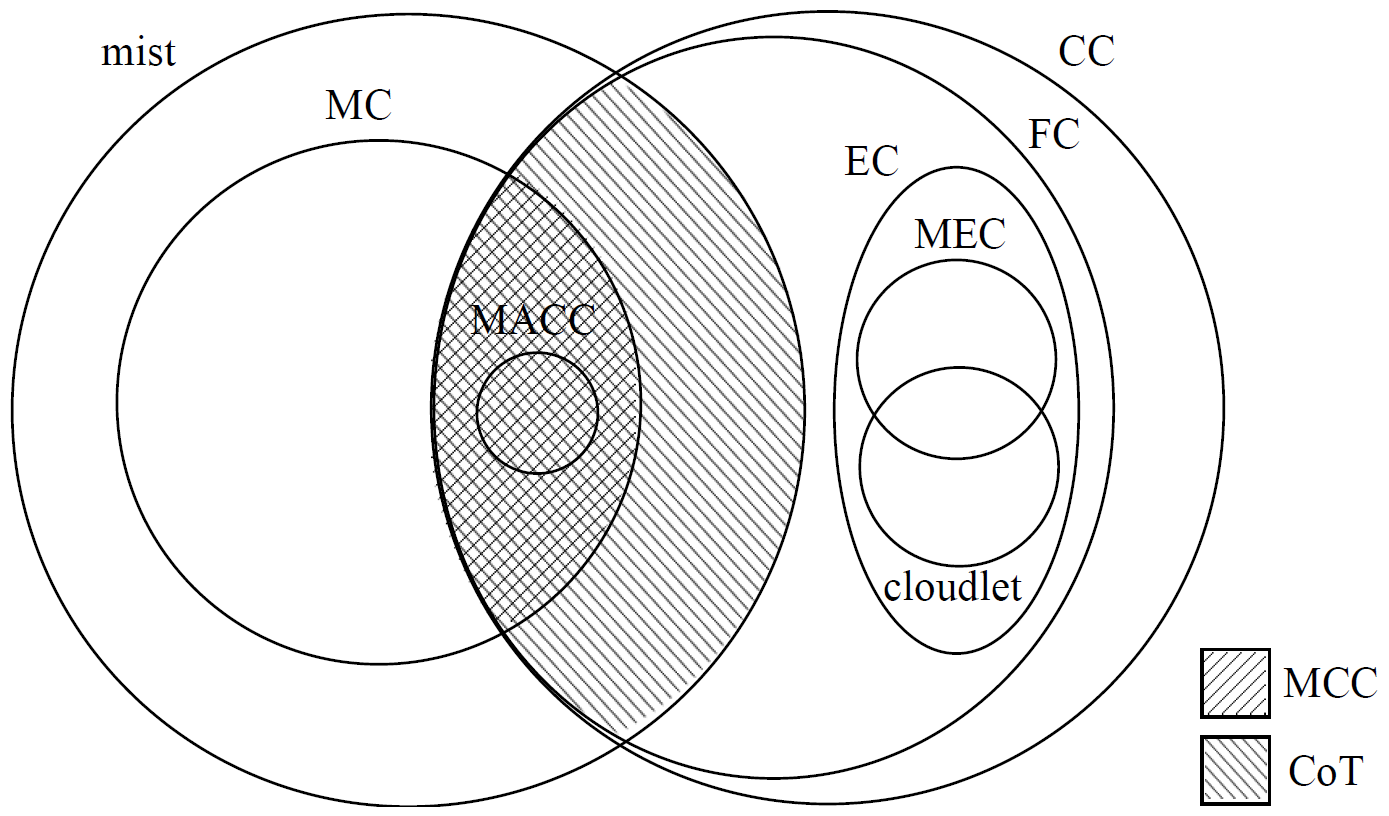
\includegraphics[width=90mm]{images/computing_paradigms}
	\caption{A classification of scope of fog computing and its related computing paradigms.}
	\label{computing_paradigms}
\end{figure}

%neste relatório consideramos que as cloudlets estão nos APs?
%falar melhor da arquitetura para explicar depois as secçoes abaixo
%A arquitetura dos Buses é boa (APs com várias cloudlets etc....)

\begin{figure}
	\centering
	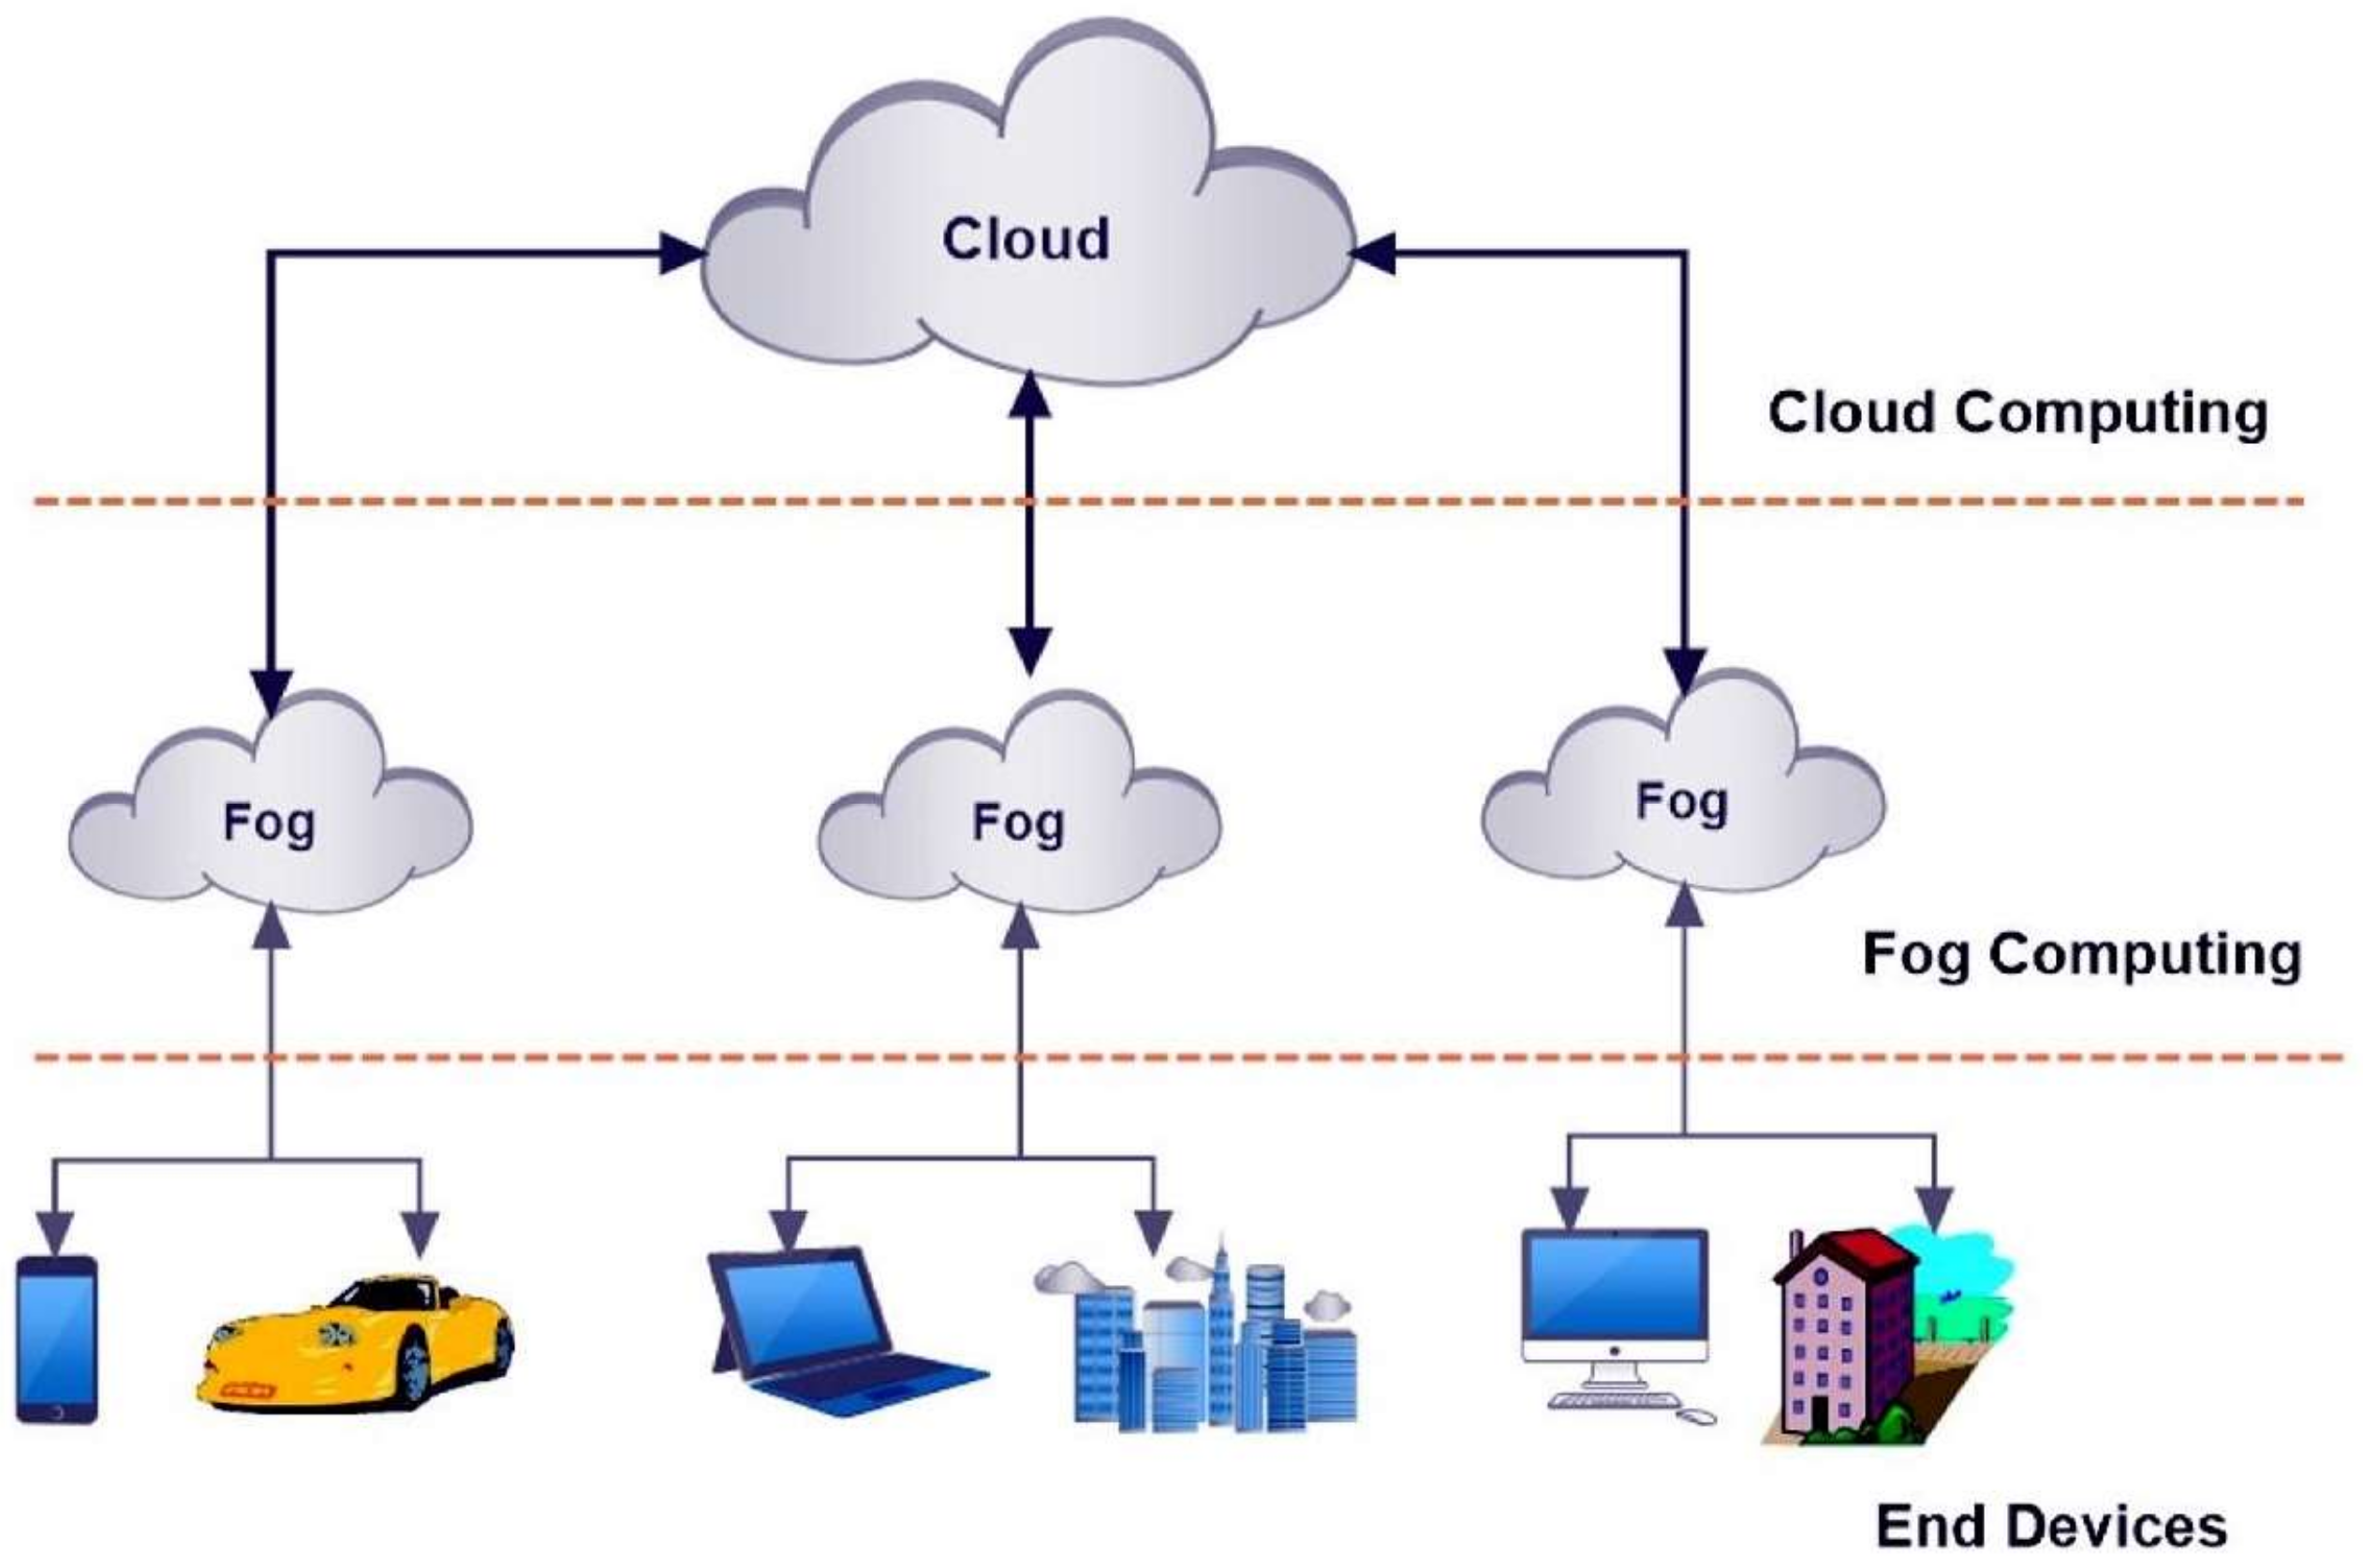
\includegraphics[width=90mm]{images/fog_architecture}
	\caption{Typical architecture of fog computing.}
	\label{fog_architecture}
\end{figure}

DESCRICAO DA ARQUITETURA DE FOG COMPUTING
which is the most typical one; a hierarchical, bi-directional computing infrastructure which consists in: a cloud, several cloudlets located at the access points (i.e. at the edge of the network) and several end devices. In this architecture, end devices communicate with cloudlets and cloudlets communicate with clouds. These cloudlets, which are capable of provide computing and storage services, can communicate with each other to perform data and process management in order to support application requirements, and to exchange fog control/management data (such as user device and application state).

In fog computing, processing and storage capacity is one hop away from the data production/consumption, which can benefit different types of applications

\begin{itemize}
	\item Applications with low latency requirements, such as pedestrian and traffic security, surveillance, applications for vision, hearing, or mobilityimpaired users, online gaming, augmented reality, and tactile computing can benefit from lower latencies because of a single hop connection to a cloudlet.
	\item Raw data collected by many devices often does not need to be transferred to the cloud for longterm storage: data can be processed, filtered, or aggregated to extract knowledge and produce reduced data sets, which in turn are to be stored; or it can be processed and utilized right-away to other edge devices in the so-called sensor/actuator loop. In both cases, the fog computing paradigm can reduce network traffic from the edge to data centers.
\end{itemize}

Cloudlets can provide reduced latencies and help in avoiding/reducing traffic congestion in the network core. However, this comes at a price: more complex and sophisticated resource management and scheduling mechanisms are needed. This raises new challenges to be overcome, e.g., dynamically deciding what, when, and where (device/fog/cloud) to carry out processing of requests to meet their quality of service requirements. Furthermore, with smart and wearable devices, such mechanisms must incorporate mobility of data sources and sinks in the fog. Traditional resource management and scheduling models for distributed systems do not consider mobility and timeliness of data production and consumption in the resource management and allocation process. Fog computing scheduling must bring users location to the resource allocation policies to uphold the benefits of fog computing proximity to the user.









\vfill\pagebreak
\subsection{Mobile Fog Computing}
\label{sec:Mobility}
Mobile Fog Computing is the ability to provide mobility support for both IoT and Fog nodes. This means that users holding end devices, can outsource the allocation and management of resources to the fog infrastructure, where both iot and fog nodes are able to move, ensuring that QoS requirements of the IoT applications are met.\\

Similar to cloud computing, fog uses the concept of virtualization. Virtualization is a vital technology at different levels. For instance, it is important to provide: (1) isolation between untrusted user-level computations, (2) mechanisms for authentication, access control, and metering, (3) dynamic resource allocation for user-level computations, (4) the ability to support a very wide range of user-level computations, with minimal restrictions on their process structure, programming languages or operating systems, (5) mobility, migration and tasks offloading mechanisms, (6) power efficiency, (7) fault tolerance.\\
\noindent\tab IoT applications may span many different operating systems and application environments (e.g., Android, iOS, Linux, Windows), as well as diverse approaches to partitioning and offloading computation. There is churn in this space from new OS versions, patches to existing OS versions, new libraries, new language runtime systems, and so on. In order to cloudlets can support all these variants, it is introduced a level of abstraction that cleanly encapsulate this messy complexity in a VM. Also, it enables VMs to coexist in a physical server (host) to share resources. Meanwhile, in fog computing the use of VMs is also crucial to provide mobility. As the end devices become more distant from the current access point, either by user or cloudlet movement, its application needs to be migrated to the most favorable access point, towards meeting its QoS (e.g., latency requirements) and improve quality of experience (QoE). This migration can be achieved through migration capabilities of VMs, which can be used to move applications and data through cloudlets according to device mobility.\\

In this context, Luiz F. Bittencourt et al. \cite{bittencourt2017mobility} took into account the same architecture shown in Fig. \ref{fog_architecture}. With the use of two applications (electroencephalography (EEG) tractor beam game to test near-real-time applications and video surveillance / object tracking application for delay-tolerant applications) to test tree different scheduling strategies (Concurrent, the First Come-First Served (FCFS), and the Delay-priority strategies), and check how scheduling decision and the change of cloudlet by the players impact the network traffic and the delays.\\

MM Lopes et al. \cite{Lopes2017} discuss resource allocation in fog computing in the face of users’ mobility, where mobility is achieved through migration of virtual machines between cloudlets. They present a new migration technique composed of two modules: migration policy which defines when the user VM should be migrated, considering aspects such as the user's speed, direction and geographical position and migration strategy, the destination cloudlet, and how the migration is performed. This work had the objective of study the impact of different migration strategies in the latency with users’ mobility.\\

[325] 2017 **Router-based brokering for surrogate discovery in edge computing.**
This paper examines the problem of discovering surrogates, which are micro-clouds, fog nodes, or cloudlets, used by client devices to offload computation tasks in a fog computing environment. In order to enable the discovery and selection of available surrogates, the authors propose a brokering mechanism in which available surrogates advertise themselves to the broker. The broker receives client requests and considers a number of attributes such as network information, hardware capabilities, and distance to find the best available surrogate for the client. The proposed mechanism is implemented on off-the-shelf home routers. They look at the problem of surrogate discovery in the context of an urban area, where they are faced with a high mobility of devices and users. Multiple brokers are interconnected using Distributed Hash Tables (DHTs) in order to exchange information. In addition, their approach introduces only a small overhead on the devices (routers) and therefore does not impede their normal function.\\

2018 **Dynamic Mobile Cloudlet Clustering for Fog Computing.**
Fog Computing is one of the solutions for offloading the task of a mobile. However the capability of fog server is still limited due to the high deployment cost. In this paper, is proposed a dynamic mobile cloudlet cluster policy (DMCCP) to use cloudlets as a supplement for the fog server for offloading. The main idea is that by monitoring each mobile device resource amount, the DMCCP system clusters the optimal cloudlet to meet the requests of different tasks from the local mobile device.\\

\noindent\tab Although several studies were already done in order to provide mobile support for IoT devices, the purpose of this study is to support mobile fog computing, once fog nodes can be anything in the path that connects things to the cloud. This distributed middle tier, in the 3-tier architecture (things-fog-cloud), can use as fog nodes any physical device that has facilities or infrastructures that can provide resources and visualization capabilities. This, may include movable fog nodes, such as cars, buses, unmanned aerial vehicles (UAVs), etc. The importance of mobile fog nodes cannot be overlooked, once they may represent a way to offload fixed cloudlet tasks and thus improve fog features. In this field there are already some early efforts.\\

Dongdong Ye et al. \cite{ye2016scalable} show a use case where buses are used as mobile cloudlets. They leverage the characteristics of buses (e.g., the same routes, many stops) and propose a scalable fog computing paradigm with servicing offloading in bus networks. The bus fog servers not only provide fog computing services for the mobile users on bus, but also are motivated to accomplish the computation tasks offloaded by roadside cloudlets. By this way, the computing capability of roadside cloudlets is significantly extended.\\

[172] 2016 **Vehicular fog computing: A viewpoint of vehicles as the infrastructures.**
Xueshi Hou et al. present the idea of utilizing vehicles as the infrastructures for communication and computation, named vehicular fog computing (VFC), which is an architecture that utilizes a collaborative multitude of end-user clients or near-user edge devices to carry out communication and computation, based on better utilization of individual communication and computational resources of each vehicle. They discussed four types of scenarios of moving and parked vehicles or congested traffic. Also, they point out the advantages against vehicular cloud computing (VCC) and the advantages in scenarios like of emergency operations for natural disaster and terrorist attack.\\

[186] 2018 **Mobile edge computing via a uav-mounted cloudlet: Optimization of bit allocation and path planning.**
Unmanned aerial vehicles (UAVs) have been considered as means to provide computing capabilities. In this model, UAVs act as fog nodes and provide computing capabilities with enhanced coverage for IoT nodes. The system aims at minimizing the total mobile energy consumption while satisfying QoS requirements of the offloaded mobile application. This architecture is based on a UAV-mounted cloudlet which provides the offloading opportunities to multiple static mobile devices. They aim to minimize the mobile energy consumption, while satisfying QoS requirements and optimize UAV’s trajectory.\\

[270] 2016 **An adaptive cloudlet placement method for mobile applications over gps big data.**
Introduces the concept of movable cloudlets and explores the problem of how to cost-effectively deploy these movable cloudlets to enhance cloud services for dynamic context-aware mobile applications. To this end, Haolong Xiang et al. propose an adaptive cloudlet placement (via GPS) method for mobile applications. Specifically, the gathering regions of the mobile devices are identified based on position clustering, and the cloudlet destination locations are confirmed accordingly. Besides, the traces between the origin and destination locations of these mobile cloudlets are also achieved.\\






%\noindent\tab Fog computing will be crucial in a diversity of scenarios. For
%instance, heterogeneous sensory nodes (e.g., sensors, controllers, actuators)
%on a self-driving vehicle, are estimated to generate about 1GB data per second
%\cite{angelica2013google}. As the number of features grow, the data deluge
%grows out of control. Moreover, these types of systems, where people's lives
%depends on it, are hard real-time what means that it is absolutely imperative
%that all deadlines are met. Offloading tasks to fog nodes will be the best
%solution, once a big effort in mobility support has been done through the
%migration of VMs using cloudlets \cite{lopes2017myifogsim}. Also, in this
%context, Puliafito et al. address three types of applications where fog is
%required, namely, citizen's healthcare, drones for smart urban surveillance and
%tourists as time travellers \cite{puliafito2017fog}, addressing the needs of
%low latency and mobility support.\\


%\subsubsection{Mobile IoT nodes} \label{subsec:MobileIoTnodes}

%\subsubsection{Mobile Fog nodes} \label{subsec:MobileFognodes}

%\subsubsection{Mobile Fog computing} \label{subsec:MobilityFog}

\subsection{Data placement}
\label{sec:Dataplacement}

%\subsubsection{Virtual Objects} \label{subsec:VirtualObjects}

%\subsubsection{Virtual Machines} \label{subsec:VirtualMachines}





















\vfill\pagebreak
\subsection{Migration Optimization}
\label{sec:Migration}
As aforementioned, in section \ref{sec:Mobility}, mobility in fog computing is supported through VM migration. Therefore, considering an environment where both users and cloudlets are mobile, the decision-making of where to send the VMs, so that users' applications have their requirements fulfilled, is a major concern is such a dynamic environment. In the section \ref{sec:Dataplacement} it was verified that applications cloud be seen as a whole, or as set of modules that may have different requirements. Regardless of their type, whenever justifies, it is necessary to re-adapt the whole system, where this is performed through the exchange of applications or modules between cloudlets, making use of VMs for this purpose. With this, it is necessary to answer the two questions: \textit{When is this exchange justified? And how is it made?}\\

\cite{ottenwalder2013migcep}
Most work studying the placement of operators in such an environment completely disregards the migration costs. However, the mobility of users requires frequent migration of operators, together with possibly large state information, to meet latency restrictions and save bandwidth in the infrastructure. In this papers, Beate Ottenwälder et al. present a placement and migration method for providers of infrastructures that incorporate cloud and fog resources. It ensures application-defined end-to-end latency restrictions and reduces the network utilization by planning the migration ahead of time using predicted mobility patterns. Furthermore, present how the application knowledge of the complex event processing (CEP) system can be used to improve current live migration techniques for Virtual Machines (VMs) to reduce the required bandwidth during the migration. First, it allows us to amortize the migration costs by selecting migration targets that ensure a low expected network utilization for a sufficiently long time. Second, it allows us to serialize the operator for the migration and migrating parts of the operator a priori in away where unnecessary events are not migrated and bandwidth is reduced.\\

\cite{urgaonkar2015dynamic}
This paper, Rahul Urgaonkar et al. present a model to optimize operational costs while providing rigorous performance guarantees as a sequential decision-making Markov Decision Problem (MDP). This model is different from the traditional solution methods (such as dynamic programming) that require extensive statistical knowledge and are computationally prohibitive. First they establish a decoupling property of the MDP that reduces it to two independent MDPs. Then, using the technique of Lyapunov optimization over renewals they design an online control algorithm that is provably cost-optimal. When the decoupling property holds, it enables the design of simple online control algorithms that do not require any knowledge of the underlying statistics of the MDPs, yet are provably optimal. This technique was applied to dynamic service migration and workload scheduling.\\

\cite{zhang2016segue}
Wuyang Zhang et al. propose SEGUE, a service that achieves optimal migration decisions by providing a long-term optimal QoS to mobile users. This model arises to overcome the limitations of previous studies that propose a static distance-based Markov Decision Process (MDP) for optimizing migration decisions that although works, it fails to consider dynamic network and server states. SEGUE is a MDP-based model which incorporates the two dominant factors in making migration decisions: 1) network state, and 2) server state. On top of that SEGUE answers the question of when to recalculate the MDP model, because to short intervals would create heavy overhead, and long intervals may translate into lazy migration. SEGUE adopts a QoS aware scheme to activate the MDP model when a QoS violation is predicted to solve for the when to migrate variable. Two components of SEGUE work together to achieve this. One module monitors network states, server workloads and user mobility and the other is responsible for QoS prediction. This allows SEGUE to avoid unnecessary migration costs and bypass any possible QoS violations.\\

\cite{ceselli2017mobile}
Alberto Ceselli et al. present a link-path formulations supported by heuristics to compute solutions in reasonable time to firstly determining where to install cloudlet facilities and secondly assigning sets of access points, such as base stations to cloudlets and lastly supporting VM orchestration and considering partial user mobility information, as well as the satisfaction of service-level agreements. Qualify the advantage in considering mobility for both users and VMs. Compare two VM mobility modes, determining that high preference should be given to live migration and bulk migration seem to be a feasible alternative on delay-stringent tiny-disk services, such as augmented reality support, and only with further relaxation on network constraints. Also, they focus on the potential medium-term planning of an edge cloud network in mobile access networks. They study two design cases: 1) network in a static state 2) network state variations in terms of load and service level, caused by user mobility.\\

\cite{sun2016primal}
User Equipment (UE) are moving in the network, and so the E2E (between UE and its Avatar) may become worse, degrading QoS. The live Avatar migration is triggered to adjust the location of the UE’s Avatar. However, the **migration process consumes extra resources** of the Avatar that may degrade the performance of applications running in the Avatar. By considering the **gain (i.e., the end-to-end delay reduction)** and the **cost (i.e., the migration overheads)** of the live Avatar (a software clone; high performance Virtual Machine (VM) located in a cloudlet) migration, Xiang Sun et al. propose a PRofIt Maximization Avatar pLacement **(PRIMAL) strategy for the cloudlet network in order to optimize the trade-off between the migration gain and the migration cost by selectively migrating the Avatars to their optimal locations.\\

\cite{abdelwahab2018clones}
Abdelwahab et al. design FogMQ, a self-deploying brokering clones that discover cloud/edge hosting platforms and autonomously migrate clones between them according to self-measured weighted tail end-to-end latency without the need of a central monitoring and control unit, not having to sacrifice computation offloading gain in cloud platforms. Finally, it is simple and requires no change in existing cloud platforms controllers.\\

\cite{Zhang2017}
One problem remains unsolved: how to distribute the work among the user device, the edge clouds, and the center cloud to meet all three requirements especially when users are mobile. Wuyang Zhang et al. propose a hybrid gaming architecture that achieves clever work distribution. It places local view change updates on edge clouds for immediate responses, frame rendering on edge clouds for high bandwidth, and global game state updates on the center cloud for user scalability. In addition, they propose an efficient service placement algorithm based on a Markov decision process. This algorithm dynamically places a user’s gaming service on edge clouds while the user moves through different access points taking into account the presence of dynamic network states and server workload states, and user mobility. However, unlike many of the service migration solutions which assumes an ignorable service transition time, they acknowledge that it is impossible to migrate an edge service from one edge to another instantly given the size of a VR game world. Therefore, they propose a mechanism to ensure a new edge cloud is activated when a player connects to the new one. It also co-places multiple users to facilitate game world sharing and reduce the overall migration overhead. Also, they derive optimal solutions and devise efficient heuristic approaches and study different algorithm implementations to speed up the runtime.\\

\cite{ye2016scalable}
In this paper, they leverage the characteristics of buses and propose a scalable fog computing paradigm with servicing offloading in bus networks. The bus fog servers not only provide fog computing services for the mobile users on bus, but also are motivated to accomplish the computation tasks offloaded by roadside cloudlets. By this way, the computing capability of roadside cloudlets is significantly extended. They consider an allocation strategy using genetic algorithm (GA). With this strategy, the roadside cloudlets spend the least cost to offload their computation tasks. Meanwhile, the user experience of mobile users are maintained.


%There are two possibilities to answer the question: \textit{when is this exchange justified?}
%In both, it is necessary to monitor the relevant system parameters, however in a different way. The first is to 



\subsection{Multi-objective}
\label{sec:Multiobjective}
QoS, QoE, Cost, Energy, Handover, Mobility, Bandwidth
\subsection{Toolkits}
\label{sec:Toolkits}



\vfill\pagebreak

%!TEX encoding = UTF-8 Unicode
\section{Description of the Project}
\label{sec:Architecture}
%- Como pensam abordar a tese tendo em conta o problema, as contribuicoes a que propoe a dar e a arquitectura definida.
%- Descricao de alto nivel da arquitectura do sistema: Arquitectura do SW explicando os principais componentes e as funcoes que executam.
%- Como procederam as escolhas das ferramentas, linguagens de programcao, ambientes de desenvolvimento, hardware
%- Como prevem desenvolver a arquitectura proposta: por onde vao comecar. Como vao integrar os componentes, que dificuldades esperam encontrar e que estrategias planeam para as ultrapassar.
\noindent Based on the reviewed works, the solution proposed in this section is to develop and implement a novel architecture which will provide mobility support to fog nodes as well as to end devices in a simulation toolkit. Besides, it will also optimize the decision-making of migration by implementing multi-objective decisions into the algorithm.\\

\subsection{Simulation toolkit}
\noindent Based on Table \ref{tab:toolkits}, it can clearly be observed that most of the existing simulation toolkits are CloudSim-based. More recent works, in fog computing, have begun to implement their investigation work in iFogSim, which is also based on CloudSim. Moreover, recently some other simulators have been proposed as extensions to iFogSim. Once such attention has been given to this ``family'' of simulators, which implies a a larger community, information and documentation, compared to other isolated simulators, our work will be based on iFogSim.\\
\noindent\tab On the one hand, iFogSim already has really fortunate characteristics. For instance, it has built-in energy (based on CPU utilization), cost (depending on memory, storage, bandwidth and CPU utilization), application (defining deadlines for modules and applications) and communication models (defining delays and bandwidth). Also, it already supports virtualization techniques, namely the use of VMs. Moreover, this simulator supports DDF programming model, where different modules may be deployed in different machines, creating dependencies between them. This is, an application module at a given machine is responsible for processing all data generated from modules hosted at machines bellow in the hierarchy. On the other hand, this simulator has some minor negative points compared with other simulators (refer to Table \ref{tab:toolkits}), however those are not critical. For example, the built-in communication model is unrealistic by disregarding low-level network issues such as link errors, congestion-related losses or management between densely collocated devices. However, these can be treated as high-level attributes like latency or bandwidth of connections. Moreover, as berofe mentioned, GreenCloud is a more fine-grained simulator in what respects to energy consumption. However in iFogSim, energy models are able to vary according to the CPU usage [implementar com envio e receção de dados!!].\\
\noindent\tab Despite the above mentioned, iFogSim still has some drawbacks, namely: it does not provide communication between fog nodes at the same level; rather it only provides parent-child communication. This feature is of most importance as discussed before (e.g., to implement an architecture based on fog colonies). Moreover it does not allow mobility of fog nodes nor end-devices and its application placement is static; does not consider any dynamic environment (although it already provides interfaces to ease this implementation).\\

\subsection{Data Placement Optimization}
\noindent Based on iFogSim, in order to achieve the desired objectives, firstly is necessary to implement ``horizontal'' communication between fog nodes.\\
\noindent\tab At the beginning of each simulation, iFogSim executes a placement strategy which is responsible to distribute the miscellaneous of modules composing an application among the available fog nodes. These nodes are deployed in a hierarchical manner where each fog node has a parent (except for the cloud). Thus, a path is composed by the intermediate fog nodes and links between them and the cloud and the gateway (fog node which is connected to the sensors and/or actuators). This strategy, favors the placement of modules closer to the end-devices (where the raw data is generated). As already mentioned modules have some dependencies (i.e. the data from one module may be the input of other model). Specifically, this strategy goes for each fog node in a given path search for what are the modules that can be placed (i.e. all their predecessors/dependencies were already placed in south fog nodes). Then, for each one of these modules, it will verify if the current node is able to host it, based on the available CPU [na memoria não? qt memoria cada modulo??]. If not, the module is transferred vertically in the hierarchy until some machine is able to host it. This is poorly efficient in terms of load balancing, QoS guarantees nor search complexity. It is worth noting that this strategy is preformed before the actual simulation begin, thus it does not take into account the real migration problems. Is a very basic static placement.\\
\noindent\tab The above strategy uses the attribute 'parent id' preform this search. Our aim is to search not only vertically but also along all neighborhoods. In a first stage, as iFogSim does not considers geographical positioning of fog servers, we will assume that fog nodes at the same level, are in the close vicinity. Once this is achieved, our objective is to somehow divide the whole system. As already mentioned this algorithm is not very efficient. It may work for systems composed by few fog nodes, but as the system grows to a bigger scale, it would not be feasible. Thus, in order to provide scalability, we aim to divide the search problem into small systems (e.g., as fog colonies does). To do so, we aim so implement graph partitioning functionality that iFogSimWithDataPlacement simulator has already implemented. Specifically this feature is implemented using three components. First, the graph modeling engine which creates an undirected graph where vertices represent fog nodes and edges model physical links. Then, the graph weighting engine that is responsible allocate weights for both vertices (based on the number of data items produced produced in each fog node) and edges (based on the number of data flows passing through these links). Finally, the graph partition engine is responsible to apply a k-way partitioning method to divide it into k sub-graphs using Metis \cite{METISSer49:online} using the typical criterias: balancing the vertex weights between sub-graphs, and minimizing the sum of cut edges weights. We also intend to compare this approaches using different criterias to perform partitioning such as the end to end latency, phisical distance or network distance (i.e. number of hops).\\
\noindent\tab After this first stage, we are now able to implement and test some algorithms proposed in the reviewed literature (refer to Section \ref{sec:Migration}). This would take into account the available parameters in iFogSim to minimize latencies and some other objectives such as energy, cost, bandwidth and, afterwards, jointly consider them all. To allow this optimization iFogSim already has built-in some valuable characteristics in fog nodes, as presented bellow:
\begin{center}
	\begin{varwidth}[t]{.5\textwidth}
	\begin{itemize}
		\item costPerSecond (Price/CPU unit)
		\item costPerMem
		\item costPerStorage
		\item costPerBw
		\item uplinkLatency
	\end{itemize}
\end{varwidth}% <---- Don't forget this %
\hspace{4em}% <---- Don't forget this %
\begin{varwidth}[t]{.5\textwidth}
	\begin{itemize}
		\item uplinkBandwidth
		\item downlinkBandwidth
		\item idlePower
		\item busyPower
	\end{itemize}
\end{varwidth}
\end{center}
As such, it will be possible to model the minimization problems and solve them with the algorithms presented in Section \ref{sec:Algoritms}. The objective is to evaluate their performance in terms of both actual optimization and computational complexity. Note that in this stage we are facing a static environment where the optimization is performed before the actual simulation.

\subsection{Mobility support}
After the above implementation, the aim is to provide mobility support. For this propose MyiFogSim, which is also an extension of iFogSim, already provide some important features. It provides mobility support to end devices through migration of virtual machines between fog nodes. On the one hand, their approach introduces the migration policy which is responsible to answer to \textit{when} the VM should be migrated using users movement (i.e. position, speed, and direction). On the other hand, upon the decision to migrate, they have introduced the migration strategy which defines \textit{where} and \textit{how} the VM should it be migrated. While the latter regards to the type of migration (i.e. non-live container/VM migration or VM live migration using post copy), the former uses some simple strategies to define the fog node destination such as shortest distance or lowest latency. However, as some review works have shown (e.g., \cite{sun2016primal,zhang2016segue}), these greedy strategies are not perfect at all, and other parameters have to be taken into account. Hence, this work intends to implement some work already preformed but not all. Besides, this work also aims to provide fog servers mobility.\\
After this implementation, is also objective to adjust the previous optimization to take into account, now, both users and fog nodes mobility and lastly to take into account mobility patterns.

\subsection{Architecture}
Based on the above mentioned our implementation consists in apply the architecture presented in figure \ref{sw_architecture}. Grey classes are from iFogSim and CloudSim simulators, yellow classes are from MyiFogSim simulator and the green ones are from iFogSimWithDataPlacement. Note that those classes are the presented in the corresponding papers, being the most important ones in their implementations. Our implementation will be focused in the white classes. It is worth mentioning that both MyiFogSim and iFogSimWithDataPlacement, as shown in Table \ref{tab:toolkits}, do not have documentation and some error were already found. Therefore, it is high unpredictable to estimate the efforts that it will require to aggregate their implementations.

\begin{figure} [t]
	\centering
	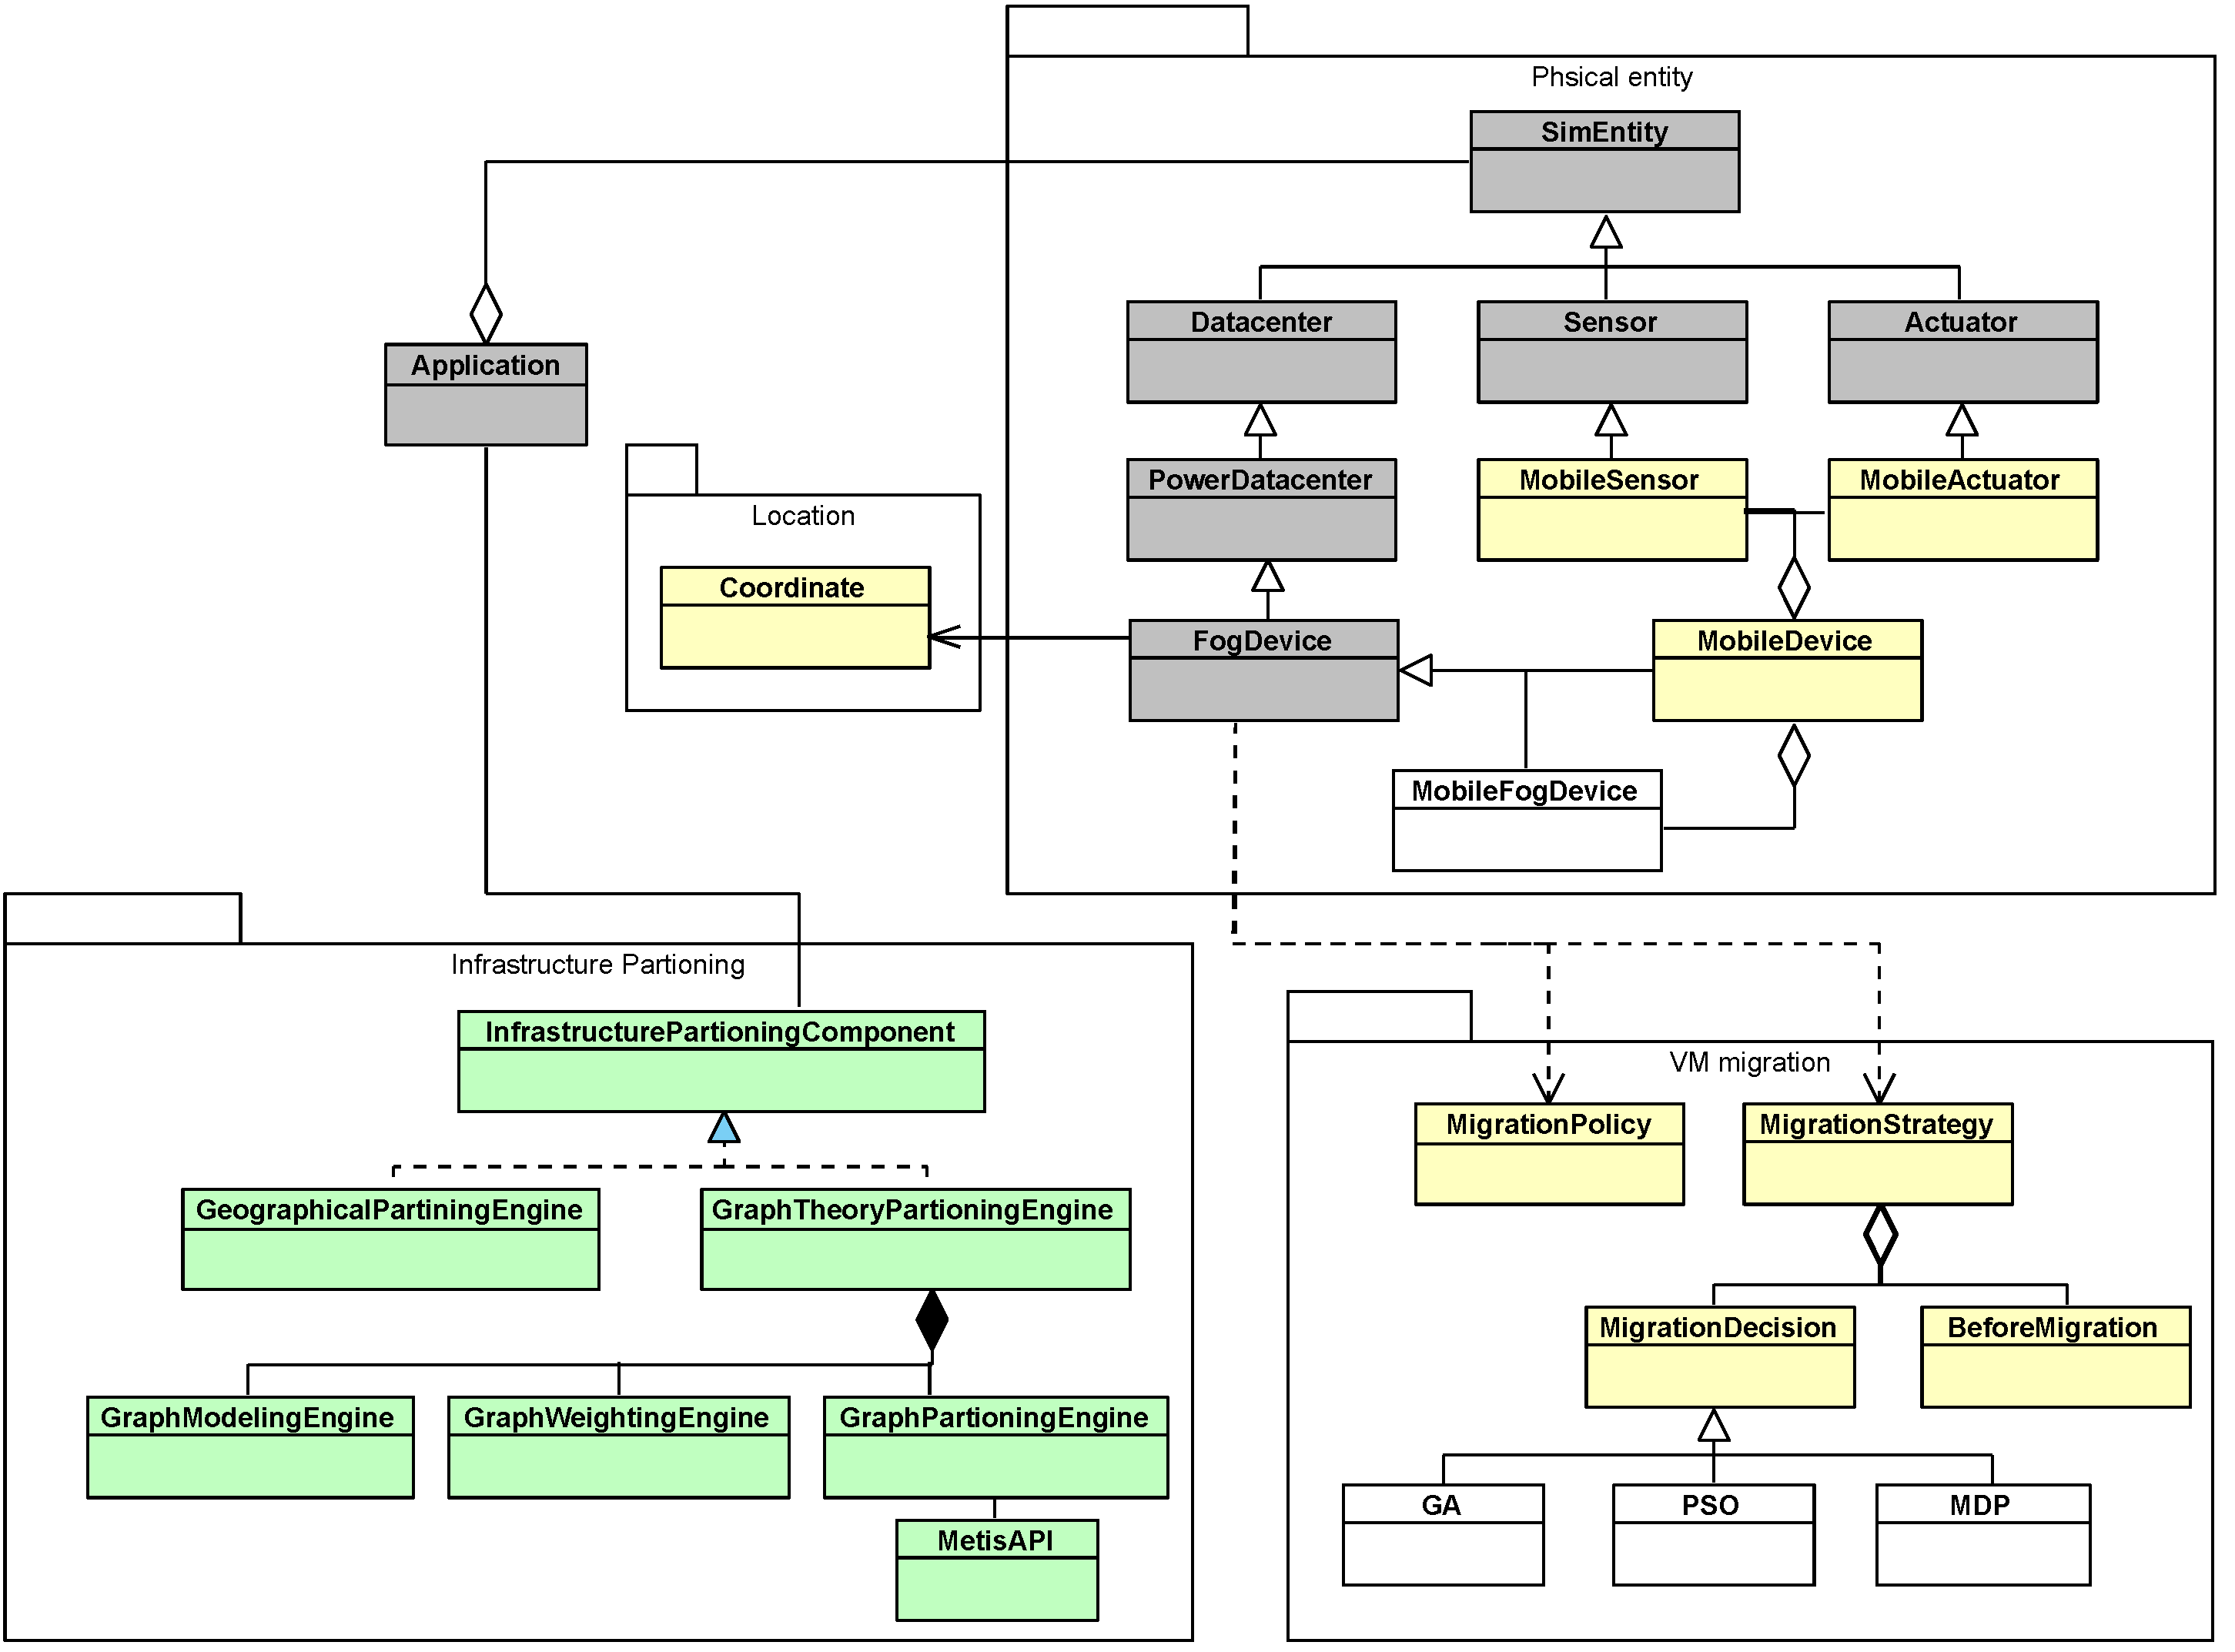
\includegraphics[width=\textwidth]{images/sw_architecture/sw_architecture}
	\caption{UML Class diagram of the main added functionalities.}
	\label{sw_architecture}
\end{figure}

As it can be seen, our work will implement four main classes, namely: MobileFogDevice, GA, PSO and MDP. The MobileFogDevice class will extend from FogDevice. Therefore, it will inherit all its attributes and methods. Besides, it will have a few similarities to the MobileDevice from MyiFogSim such as the direction, speed and geographical position. The three latter will focus on implementing the algoritms of optimization explained in Section \ref{sec:Migration}. Relatively to the recalculation of the optmization problem, it cannot be defined how it will be done now. This is because, we first need to evaluate their behavior in terms of computational complexity and execution time. Only after this process we will be able to define it. However there are some options to do so. Based on the review literature we have three options. The first, proposed by MyiFogSim, is to recalculate only when the user is predicted to go out of range from a base station. Based on its position, direction and speed we can predict an handover. When this is verified, the algorithm is executed to compute the best placement to its VM (compute the cloudlet destination). Their approach is a single user-centric approach, therefore it does not take into account system efficiency what is a bad approach as already explained. Other options were already proposed in the literature. For instance, the algorithm may be recalculated periodically, but the optimal time interval is never proposed (it is only said that it depends on system dynamics). Finally, the third approach, it to only recalculate when a QoS violation is predicted. In the latter, it would evolve several parameters such as server and network states as well as mobility and request patterns. As already stated, there are quite unpredictable time implementations during the implementation of the proposed architecture. Therefore, we do not know if it will be possible to implement mobility and request patterns and we may be restricted to the first two approaches.\\

\subsection{Optimization Algoritms}
As already mentioned, we intend to implement and test some of the proposed algorithms in the reviewed literature. From the panoply of solvers, we intend to study the behavior of the three presented bellow and, later, depending on the time available, more algorithms may be tested.

\subsubsection{Genetic Algorithm}
GA is an adaptive heuristic search algorithm. It is based on the idea of natural selection and genetics. Specifically, it is an iterative random search which is able to provide high-quality solutions for optimization problems and search problems.\\
\noindent\tab The algorithm has an arbitrary number of individuals composing the population. During the process, each iteration is characterized by a generation of individuals (whith the same size of population), representing a point in search space and possible solution. Yet, for each iteration, it is simulated the process of natural selection or ``survival of the fittest''. Each individual has a chromosome with genes. By evaluate them, it is possible to define its fitness score. Using this score, there are three operations in the creation of the next generation, namely: the selection operator which selects the individuals that will be part of the next generation, the crossover operator which represents mating between two individuals, resulting in a new individual with a chromosome composed by random genes from the two parents, and, finally, the mutation operator that will randomly introduce genes in the individuals resulting from the crossover operator to maintain the diversity in population to avoid the premature convergence \cite{whitley1994genetic}.

\subsubsection{Particle Swarm Optimization}

\subsubsection{Markov Decision Process}

%A arquitetura dos Buses é boa (APs com várias cloudlets etc....)

%Starting from available simulators a significant programming effort is required to obtain a simulation tool meeting the actual needs.
%Simply applying existing radio access-oriented MM (mobility management) schemes leads to poor performance mainly due to the co-provisioning of radio access and computing services of the MEC-enabled (mobile edge computing) BSs (base stations).
%On a self-driving vehicle, are estimated to generate about 1GB data per second \cite{angelica2013google}. As the number of features grow, the data deluge grows out of control. Moreover, these types of systems, where people's lives depends on it, are hard real-time what means that it is absolutely imperative that all deadlines are met. Offloading tasks to fog nodes will be the best solution, once a big effort in mobility support has been done through the migration of VMs using cloudlets \cite{lopes2017myifogsim}. Also, in this context, Puliafito et al. address three types of applications where fog is required, namely, citizen's healthcare, drones for smart urban surveillance and tourists as time travellers \cite{puliafito2017fog}, addressing the needs of low latency and mobility support.\\
%!TEX encoding = UTF-8 Unicode
%- Como pensam testar a solucao e validar a vossa idea, que processo vao
%  utilizar durante o desenvolvimento para facilitar a rrealizacao de testes e a
%  recolha de resultados.
%- Pretendo usar um prototipo: que equipamentos/linguagens de programacao a usar
\section{Evaluation}
\label{sec:Evaluation}

The evaluation of the proposed architecture will be done xxxx
%!TEX encoding = UTF-8 Unicode
\section{Schedule of Future Work}
\label{sec:Schedule}

Future work is scheduled as follows:
\begin{itemize}
  \item Choice of applications and specifications of test target scenarios;[??]
  \item Communication between fog nodes at the same level; [15 dias]
  \item Write the dissertation about the work performed;[1mes depois do inicio - fim]
  \item Static Optimization; [1 mes]
  \item Preliminary results; [2 sem (comeca uma semada antes do fim do Static Optimization)]
  \item Mobility implementation; [1 mes]
  \item Optimization with mobility; [3 sem]
  \item Final results. [2 sem (comeca uma semada antes do fim do Optimization with mobility)]
\end{itemize}

%!TEX encoding = UTF-8 Unicode
\section{Conclusion}
\label{sec:Conclusion}
%Fazer o resumo do trabalho efectuado, retomando a idea, as contribuicoes definidas e a forma como estas se materializam.

xxxxx 



\bibliographystyle{IEEEtran}
\bibliography{./references/report}

\end{document}
